\documentclass{article}
\usepackage[utf8]{inputenc}
\usepackage{amssymb}
\usepackage{amsfonts}
\usepackage{amsmath}
\usepackage[utf8]{inputenc}
\usepackage[norsk]{babel}
\usepackage{lmodern}
\usepackage{float}
\usepackage{graphicx}
\DeclareGraphicsExtensions{.pdf,.png,.jpg}
\usepackage{latexsym}
\usepackage{hyperref}
\usepackage[euler]{textgreek}
\usepackage{stackengine}
\usepackage[version-1-compatibility]{siunitx}
\usepackage{pdfpages}
\usepackage{fixltx2e}
\hypersetup{pdfborder={0 0 0}}
\usepackage{pgfplots}
\pgfplotsset{compat=newest}
\pgfplotsset{plot coordinates/math parser=false}
\newlength\figureheight
\newlength\figurewidth
\usepackage[section]{placeins}%Sørger for at plots og andre floats holder seg til sin section.
\setlength\parindent{0pt}%Setter indent til 0



\title{Exercise 1 - TTK4130 Modeling and Simulation}
\author{Camilla Sterud}
\date{}

\begin{document}

\maketitle

\newpage

\section{Problem 1}

\begin{align}
	Ni = \phi(\mathcal R_a + \mathcal R_c + \mathcal R_b + \mathcal R_r).\label{eq:Ni}\\ 
	\mathcal R_a = \frac{z}{A\mu_0}, \mathcal R_r = const. \label{eq:R_a} \\ 
	\mathcal R_c, \mathcal R_b << \mathcal R_r, \mathcal R_a. \label{eq:small}
\end{align}


\subsection{a}

\begin{equation}\label{eq:R_r}
	\mathcal R_r = \frac{z_0}{A\mu_0}, z_0 = const.
\end{equation}

Using Equation \ref{eq:Ni} together with the relations from equations \ref{eq:R_a} and \ref{eq:R_r} we get

\begin{equation*}
	Ni = \phi(\frac{z}{A\mu_0} + \mathcal R_c + \mathcal R_b + \frac{z_0}{A\mu_0}).
\end{equation*}

Since $\mathcal R_c$ and $\mathcal R_b$ are neligible (Equation \ref{eq:small}), the total magnetomotive force on the ball is

\begin{equation*}
	\underline{\underline{Ni = \frac{\phi}{A\mu_0}(z + z_0).}}
\end{equation*}

\subsection{b}

\begin{equation} \label{eq:induct}
	L(z) = \frac{N\phi}{i} = \frac{N^2A\mu_0}{z + z_0}.
\end{equation}

\begin{equation}\label{eq:magnF}
	F = \frac{i^2}{2}\frac{\partial L(z)}{\partial z}.
\end{equation}

Assume positive direction downwards and gravitational acceleration $g$.

\begin{align*}
	ma = \Sigma F\\
	m\ddot z = mg + F\\
	m\ddot z = mg + \frac{i^2}{2}N^2A\mu_0(z + z_0)^{-2}.
\end{align*}

\begin{equation}\label{eq:motion}
	\underline{\underline{\ddot z = g - \frac{1}{2m}i^2N^2A\mu_0(z+z_0)^{-2}}}
\end{equation}


\subsection{c}
Linearizing about $z_d$, $\dot z_d = 0$, $\ddot z_d = 0$.
\begin{align*}
	0 = g - \frac{1}{2m}i_d^2N^2A\mu_0(z_d+z_0)^{-2}\\
	i_d = \frac{1}{N}\sqrt{\frac{2mg}{A\mu_0}}(z_d + z_0)
\end{align*}

Equation \ref{eq:motion} we now call $f_1$. We define $z = z_d + \Delta z, i = i_d + \Delta i$ and thereby $\dot z = \Delta\dot z$. A Linearization of Equation \ref{eq:motion} around the point $z_d$ is then


	$\Delta\ddot z = \left. \frac{\partial f_1}{\partial \dot z} \right.\Bigg|_{\shortstack{\tiny $z = z_d$ \\ \tiny $\dot z = \dot z_d$ \\ \tiny $i = i_d$}} \Delta \dot z + \left. \frac{\partial f_1}{\partial z} \right.\Bigg|_{\shortstack{\tiny $z = z_d$ \\ \tiny $\dot z = \dot z_d$ \\ \tiny $i = i_d$}} \Delta z + \left. \frac{\partial f_1}{\partial i} \right.\Bigg|_{\shortstack{\tiny $z = z_d$ \\ \tiny $\dot z = \dot z_d$ \\ \tiny $i = i_d$}} \Delta i\\$

\begin{equation*}
	\Delta\ddot z = \frac{1}{m}i_d^2N^2A\mu_0(z_d+z_0)^{-3} \Delta z - \frac{1}{2m}i_dN^2A\mu_0(z_d+z_0)^{-2}\Delta i
\end{equation*}


\begin{equation*}
	\underline{\underline{\Delta \ddot z = \frac{2g}{z_d + z_0} \Delta z - \frac{N}{z_d + z_0}\sqrt{\frac{2gA\mu_0}{m}} \Delta i}}
\end{equation*}


\newpage
\section{Problem 2}

\subsection{b}

Natural signal-flow inputs are $T_i$ and $\omega_{i-1}$. The outputs should be $T_{i-1}$ and $\omega_i$. For natural energy-flow, inputs should be $T_{i-1}$ and $\omega{i-1}$, with $T_i$ and $\omega_i$ as outputs. 

\subsection{c}

\begin{figure}[!ht]
    \centering
    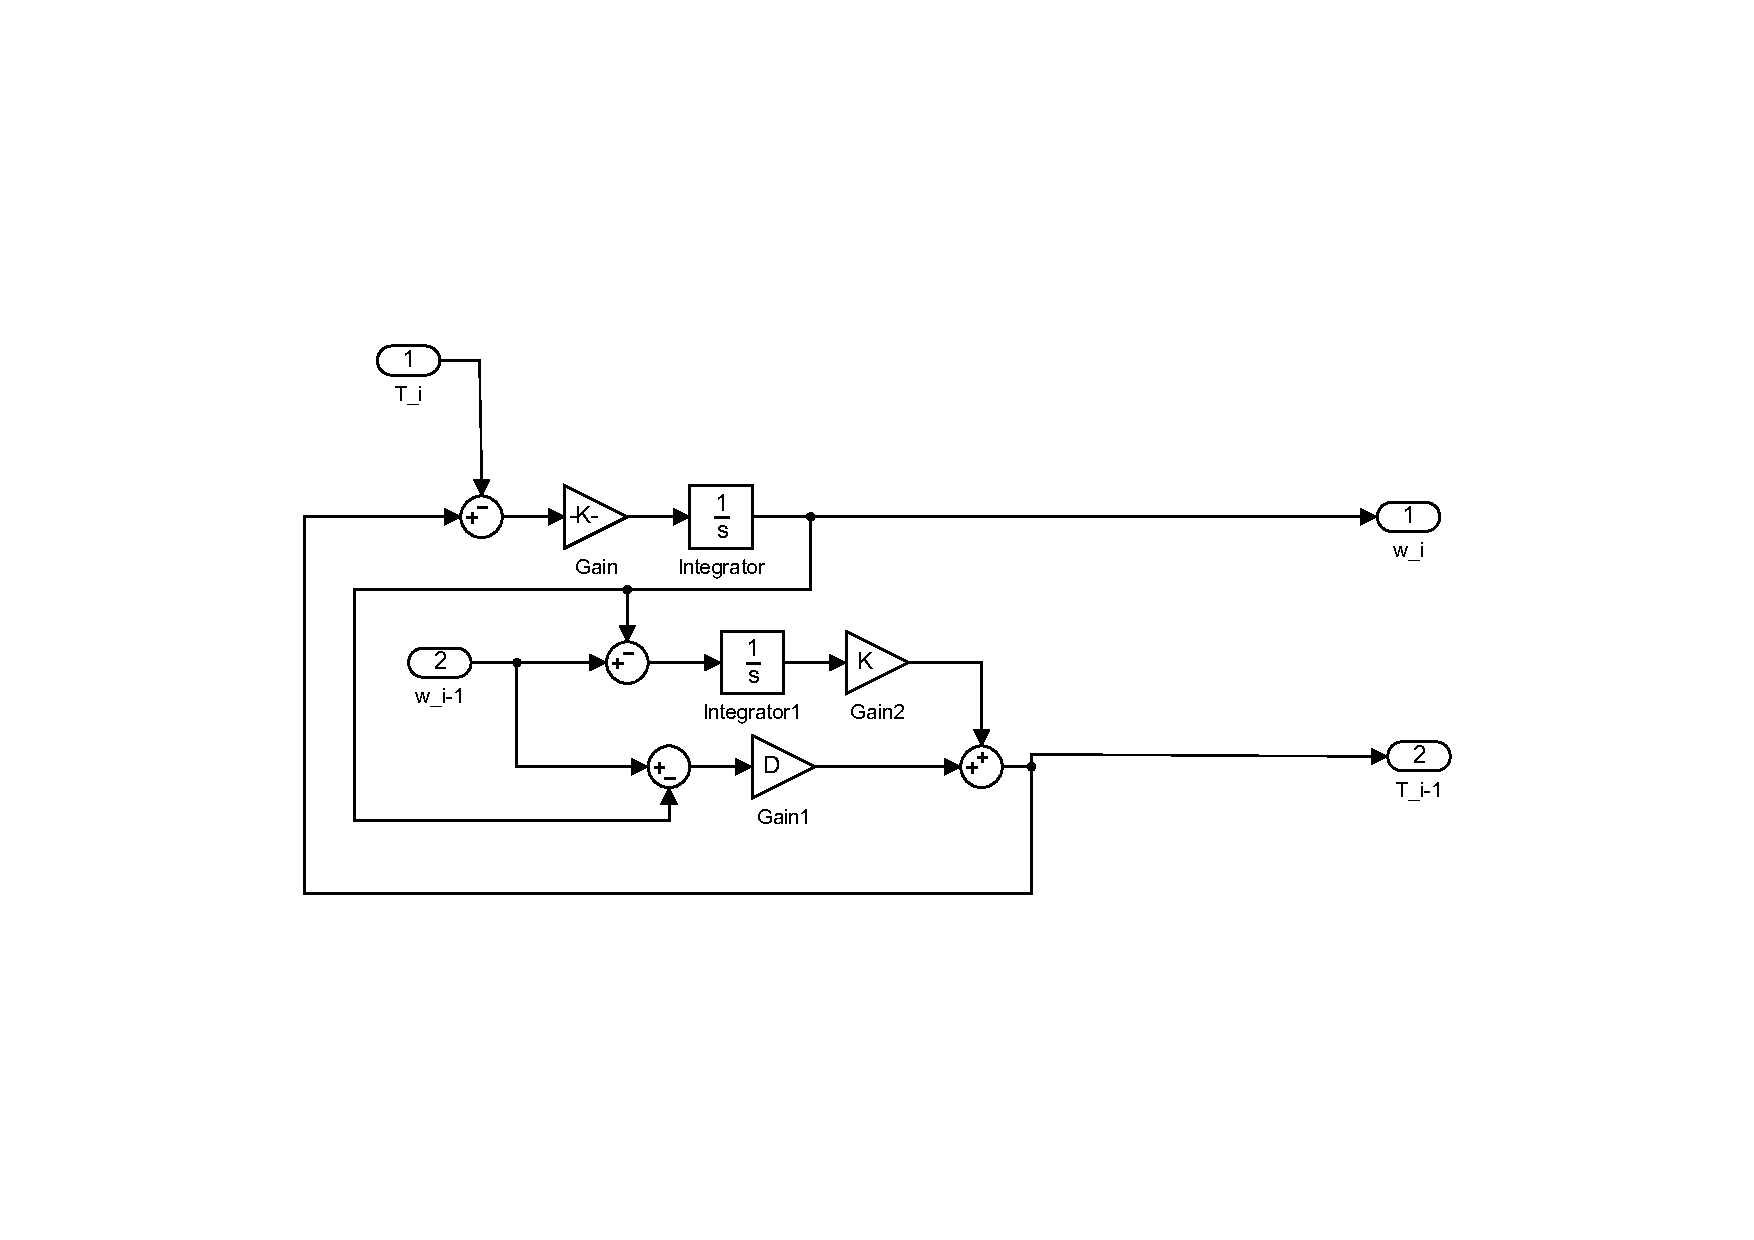
\includegraphics[width = \textwidth]{ex1_2_elasticload}
    \caption{The elastic load implemented in Simulink}
    \label{fig:elasticload} 
\end{figure}

\subsection{d}

\begin{figure}[!ht]
    \centering
    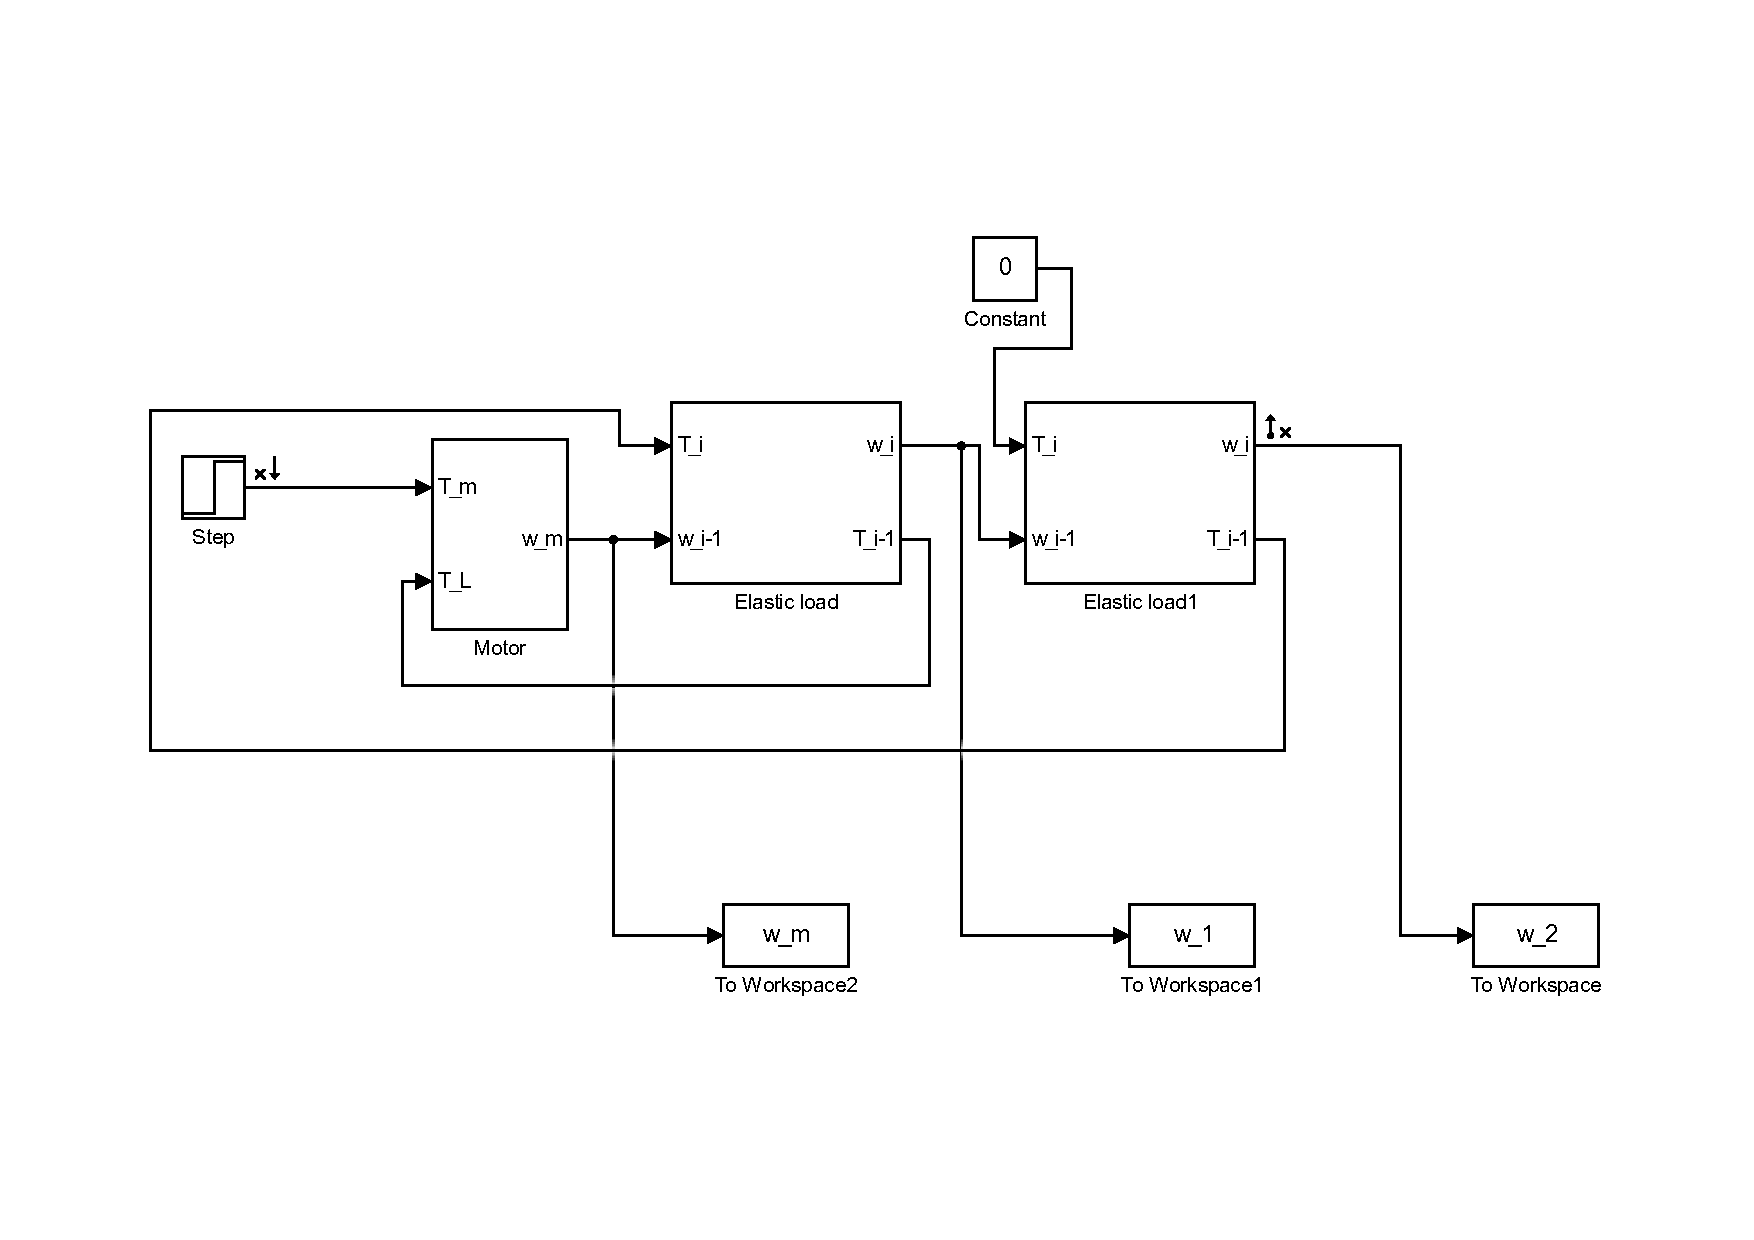
\includegraphics[width = \textwidth]{ex1_2}
    \caption{Two elastc loads in series with the motor.}
    \label{fig:twoloads} 
\end{figure}

\begin{figure}[!ht]
    \centering
    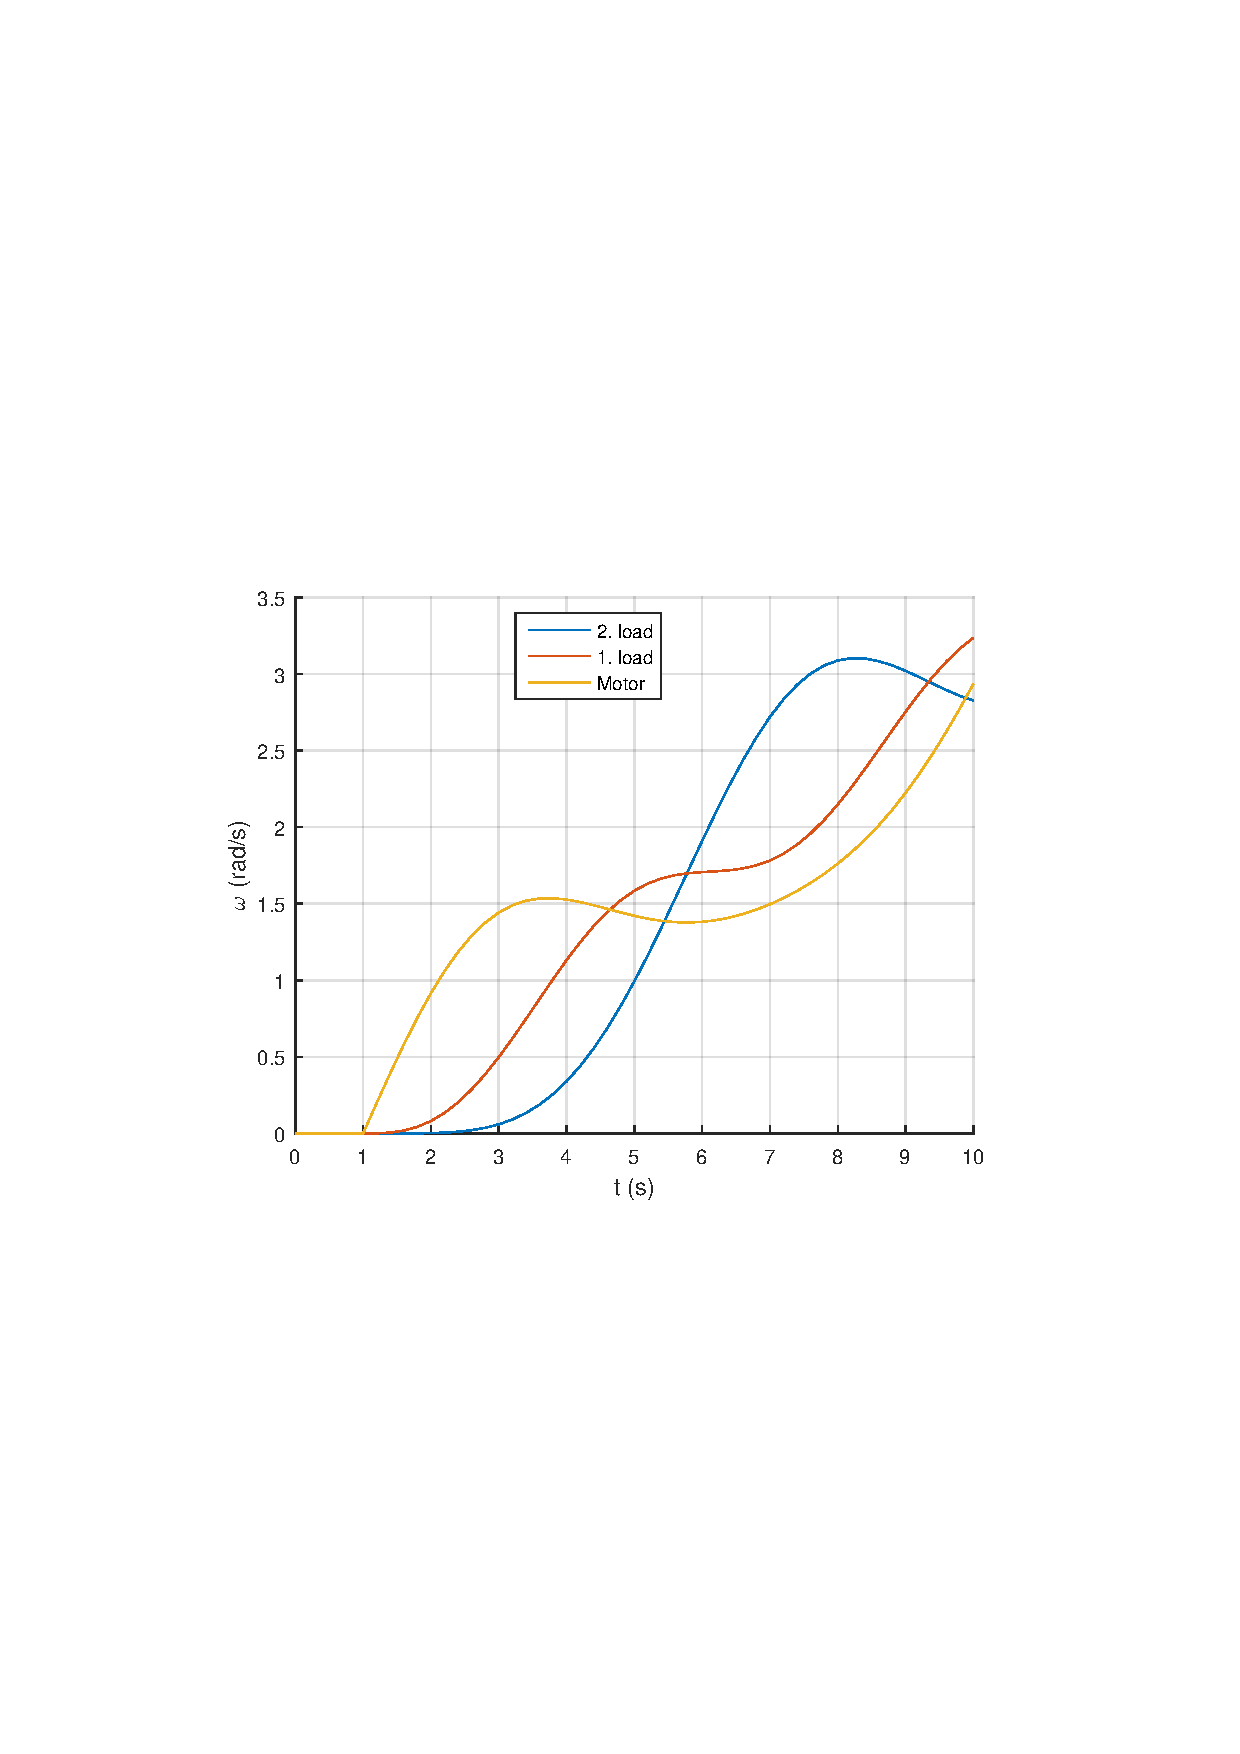
\includegraphics[width = \textwidth]{ex1_2b}
    \caption{Plot of the rotational velocity of the motor and the two loads.}
    \label{fig:veloplot} 
\end{figure}

As seen in Figure \ref{fig:veloplot}, the angular velocity of the second load is delayed. This is due to the phase displacement between the motor and the first load, and the first and the second load. 

\subsection{e}

\begin{figure}[!ht]
    \centering
    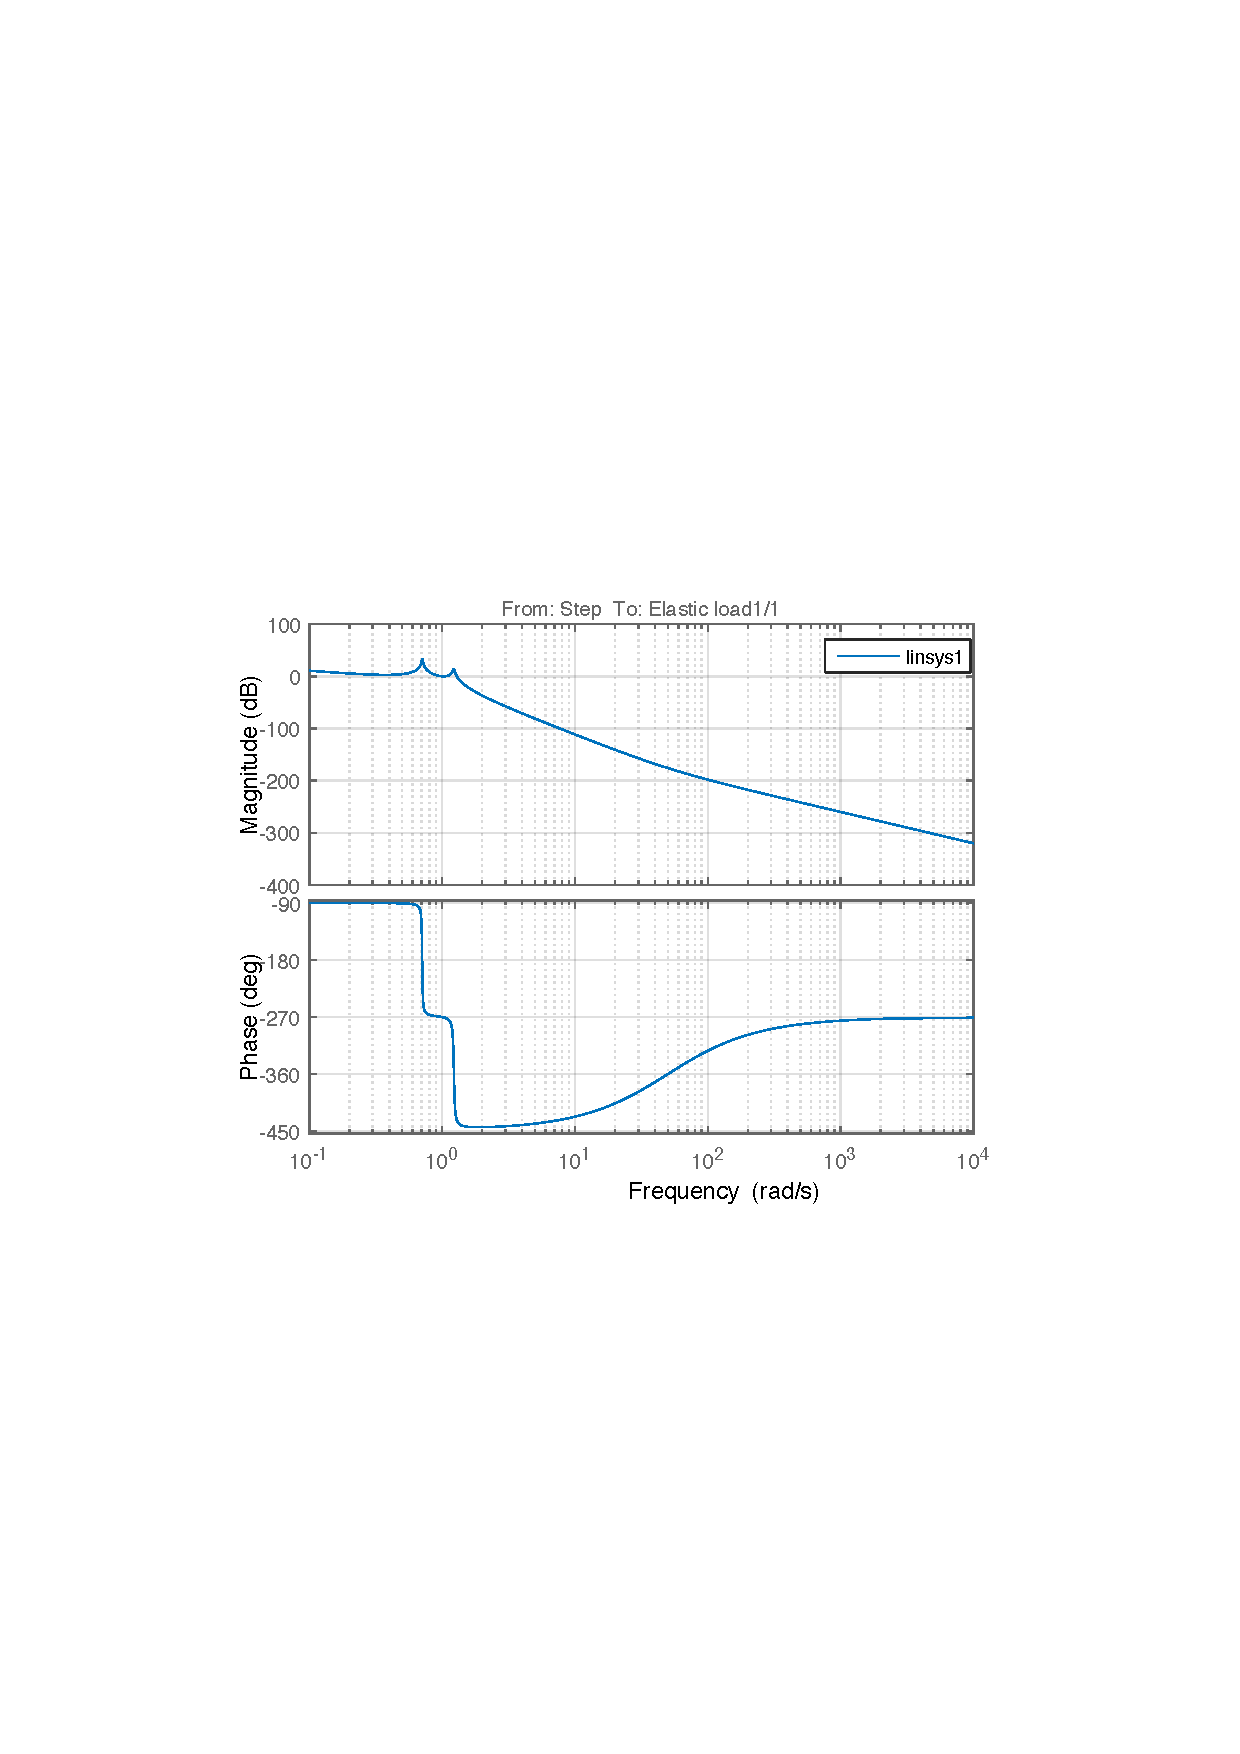
\includegraphics[width = \textwidth]{ex1_2_bode}
    \caption{Bode plot of the transfer function from the step input to the rotational velocity of the second load.  Made in with Simulink's linear analysis.}
    \label{fig:bodeSimu} 
\end{figure}

In the bode plot in Figure \ref{fig:bodeSimu} it is clear that the system has two resonance peaks at $\omega = \SI[per-mode=fraction]{1.5}{\rad\per\second}$ and $\omega = \SI[per-mode=fraction]{0.7}{\rad\per\second}$. For small frequencies the effects of integrators are present, which causes the phase to fall almost down to $-450$. For large frequencies, the amplification of the input signal is small, and the phase stabilizes at about $\SI{-270}{\degree}$

\newpage

\section{Problem 3}

\subsection{a}

The rotational speed of the second load when simulated using Modelica can be seen in Figure \ref{fig:dymola1}. It looks just the same as when using Simulink (Figure \ref{fig:veloplot}).

The graphical view in Dymola gives a lot more visual information than the one in Simulink. By just looking at the model it is possible to understand what is to be simulated, while in Simulink you have to know and understand the mathematical model to get what is going on. 

\begin{figure}[h]
    \centering
    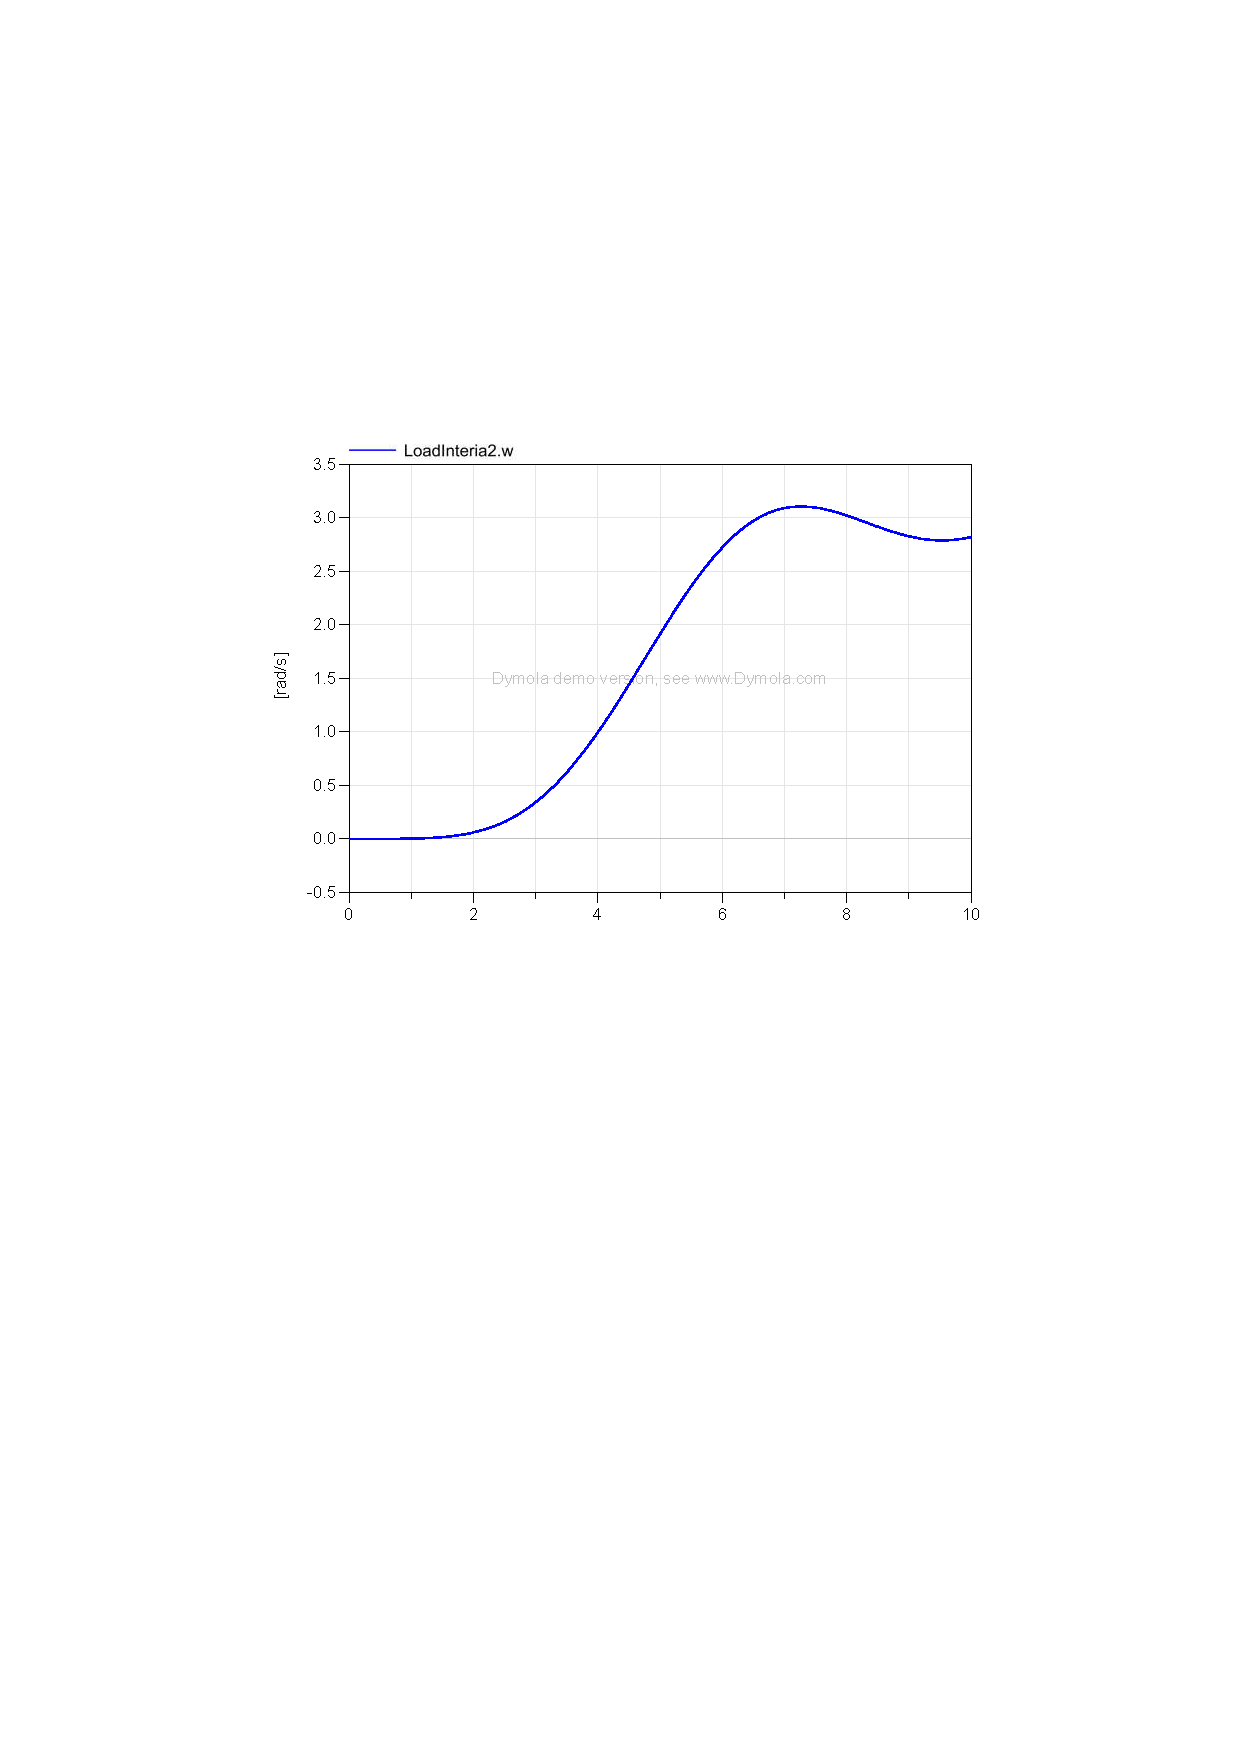
\includegraphics[width = \textwidth]{ex1_3a}
    \caption{The rotational velocity of the second load when simulated using Dymola.}
    \label{fig:dymola1} 
\end{figure}

\subsection{b}
The Flange\_a object in Dymola is a component that connects rotating mechanical systems. This can be compared to the input/ouput ports of Simulink subsystems. They both comminicate with the outer system, but while the Simulink ports are purely objects to hold numbers, the Flange\_a also holds physical attributes (rotation angle and torque). The Flange\_a is a part of the simulation and emulates a physical connection, while Simulink ports merely are there to communicate with outer subsystems. 


\subsection{c}

The bode plot created using Dymolas linear analysis tools can be seen in Figure \ref{fig:bodeDymola}. It looks very much the same as the one created with SImulink (Figure \ref{fig:bodeSimu}).

\begin{figure}[h]
    \centering
    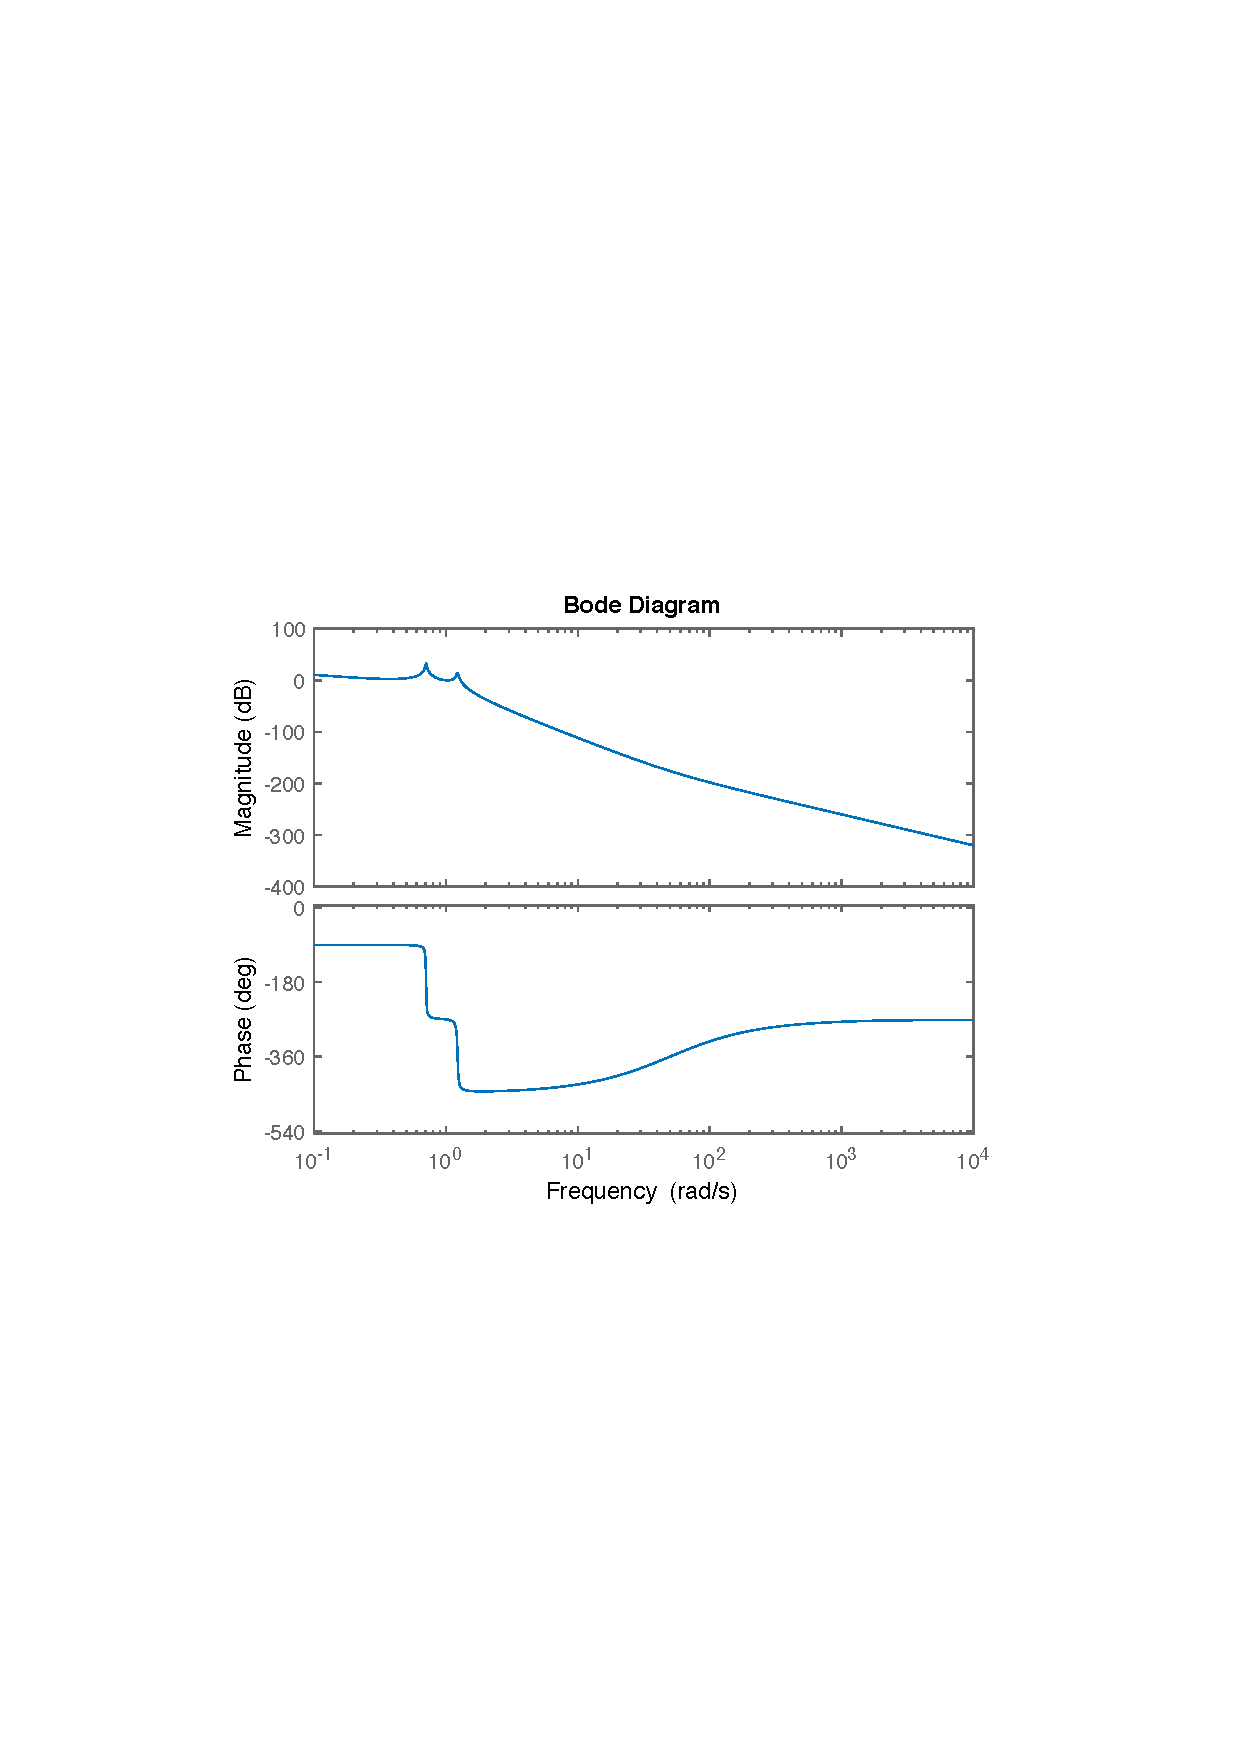
\includegraphics[width = \textwidth]{ex1_3c_bode}
    \caption{Bode plot of the system when linearized with Dymola.}
    \label{fig:bodeDymola} 
\end{figure}



\end{document}